\documentclass{article} % A4 paper and 11pt font size
\setcounter{secnumdepth}{0}

\usepackage{amssymb, amsmath, amsfonts}
\usepackage{moreverb}
\usepackage{graphicx}
\usepackage{enumerate}
\usepackage{graphics}
\usepackage[margin=1.25in]{geometry}
\usepackage{color}
\usepackage{tocloft}
\renewcommand{\cftsecleader}{\cftdotfill{\cftdotsep}}
\usepackage{array}
\usepackage{float}
\usepackage{hyperref}
\usepackage{textcomp}
\usepackage[makeroom]{cancel}
\usepackage{bbold}
\usepackage{alltt}
\usepackage{physics}
\usepackage{mathtools}
\usepackage[normalem]{ulem}
\usepackage{amsthm}
\usepackage{tikz}
\usetikzlibrary{positioning}
\usetikzlibrary{arrows}
\usepackage{pgfplots}
\usepackage{bigints}
\allowdisplaybreaks
\pgfplotsset{compat=1.12}

\theoremstyle{plain}
\newtheorem*{theorem*}{Theorem}
\newtheorem{theorem}{Theorem}
\newtheorem*{lemma*}{Lemma}
\newtheorem{lemma}{Lemma}

\newenvironment{definition}[1][Definition]{\begin{trivlist}
\item[\hskip \labelsep {\bfseries #1}]}{\end{trivlist}}

\newcommand{\E}{\varepsilon}
\def\Rl{\mathbb{R}}
\def\Cx{\mathbb{C}}

\newcommand{\Ei}{\text{Ei}}

\usepackage[T1]{fontenc} % Use 8-bit encoding that has 256 glyphs
\usepackage{fourier} % Use the Adobe Utopia font for the document - comment this line to return to the LaTeX default
\usepackage[english]{babel} % English language/hyphenation

\usepackage{sectsty} % Allows customizing section commands
\allsectionsfont{\centering \normalfont\scshape} % Make all sections centered, the default font and small caps

\usepackage{fancyhdr} % Custom headers and footers
\pagestyle{fancy} % Makes all pages in the document conform to the custom headers and footers
\fancyhead[L]{\bf Sam Fleischer}
\fancyhead[C]{\bf UC Davis \\ Applied Mathematics (MAT207C)} % No page header - if you want one, create it in the same way as the footers below
\fancyhead[R]{\bf Spring 2016}

\fancyfoot[L]{\bf } % Empty left footer
\fancyfoot[C]{\bf \thepage} % Empty center footer
\fancyfoot[R]{\bf } % Page numbering for right footer
\renewcommand{\headrulewidth}{0pt} % Remove header underlines
\renewcommand{\footrulewidth}{0pt} % Remove footer underlines
\setlength{\headheight}{25pt} % Customize the height of the header

\newcommand{\VEC}[2]{\left\langle #1, #2 \right\rangle}
\newcommand{\ran}{\text{\rm ran }}
\newcommand{\Hilb}{\mathcal{H}}

\DeclareMathOperator*{\esssup}{\text{ess~sup}}

\newcommand{\problem}[2]{
\vspace{.375cm}
\boxed{\begin{minipage}{\textwidth}
    \section{\bf #1}
    #2
\end{minipage}}
}

\numberwithin{equation}{section} % Number equations within sections (i.e. 1.1, 1.2, 2.1, 2.2 instead of 1, 2, 3, 4)
\numberwithin{figure}{section} % Number figures within sections (i.e. 1.1, 1.2, 2.1, 2.2 instead of 1, 2, 3, 4)
\numberwithin{table}{section} % Number tables within sections (i.e. 1.1, 1.2, 2.1, 2.2 instead of 1, 2, 3, 4)

\setlength\parindent{0pt} % Removes all indentation from paragraphs - comment this line for an assignment with lots of text

\newcommand{\horrule}[1]{\rule{\linewidth}{#1}} % Create horizontal rule command with 1 argument of height

\usepackage{xcolor}
\definecolor{light-gray}{gray}{0.9}

\title{ 
\normalfont \normalsize 
\textsc{UC Davis, Applied Mathematics (MAT207C), Spring 2016} \\ [25pt] % Your university, school and/or department name(s)
\horrule{2pt} \\[0.4cm] % Thin top horizontal rule
\Huge Homework \#1 \\ % The assignment title
\horrule{2pt} \\[0.5cm] % Thick bottom horizontal rule
}

\author{\huge Sam Fleischer} % Your name

\date{April 8, 2016} % Today's date or a custom date

\begin{document}\thispagestyle{empty}

\maketitle % Print the title

\makeatletter
\@starttoc{toc}
\makeatother

\pagebreak

%%%%%%%%%%%%%%%%%%%%%%%%%%%%%%%%%%%%%%
\problem{Problem 1}{
Find the two-term asymptotic expansion for small $\E$ for all real roots $x$ of the below equations.
\begin{enumerate}[(a)]
    \item $\E^2 x^3 - x + \E = 0$
    \item $\E \exp(x^2) = 1 + \dfrac{\E}{1 + x^2}$
\end{enumerate}}








%%%%%%%%%%%%%%%%%%%%%%%%%%%%%%%%%%%%%%
\problem{Problem 2}{
The Exponential integral function is defined as $$\Ei(x) = \int_x^\infty \frac{\exp(-s)}{s} \dd s.$$  Derive an asymptotic expansion for $\Ei(x)$ for large $x$.  Use a computer (e.q.~$\text{expint}(x)$ in MATLAB) to check the accuracy of your expansion for different values of $x$ and for different numbers of terms.  Discuss your results.
}

By integration by parts,
\begin{align*}
    \int_x^\infty \frac{\exp(-s)}{s}\dd s &= \left.\frac{-\exp(-s)}{s}\right|_x^\infty - \int_x^\infty \frac{\exp(-s)}{s^2}\dd s \\
    &= \frac{\exp(-x)}{x} - \qty[\left.\frac{-\exp(-s)}{s^2}\right|_x^\infty - 2\int_x^\infty \frac{\exp(-s)}{s^3}\dd s] \\
    &\vdots \\
    &= \exp(-x)\qty[\frac{(-1)^0 0!}{x} + \frac{(-1)^1 1!}{x^2} + \frac{(-1)^2 2!}{x^3} + \dots + \frac{(-1)^n n!}{x^{n+1}}] + R_n(x)
\end{align*}
where
\begin{align*}
    R_n(x) = (-1)^{n+1}(n+1)!\int_x^\infty \frac{\exp(-s)}{s^{n+2}}\dd s
\end{align*}
Thus the asymptotic expansion for $\Ei(x)$ for large $x$ is
\begin{align*}
    \Ei(x) \sim \exp(-x)\sum_{n=0}^\infty \frac{(-1)^n n!}{x^{n+1}}.
\end{align*}
This is a divergent series in $n$, but converges to $0$ as $x \rightarrow \infty$ when $n$ is fixed.  The following graph shows the error between the asymptotic expansion and the exponential integral function, as calculated by MATLAB and graphed in Python.
\begin{figure}[ht!]
    \centering
    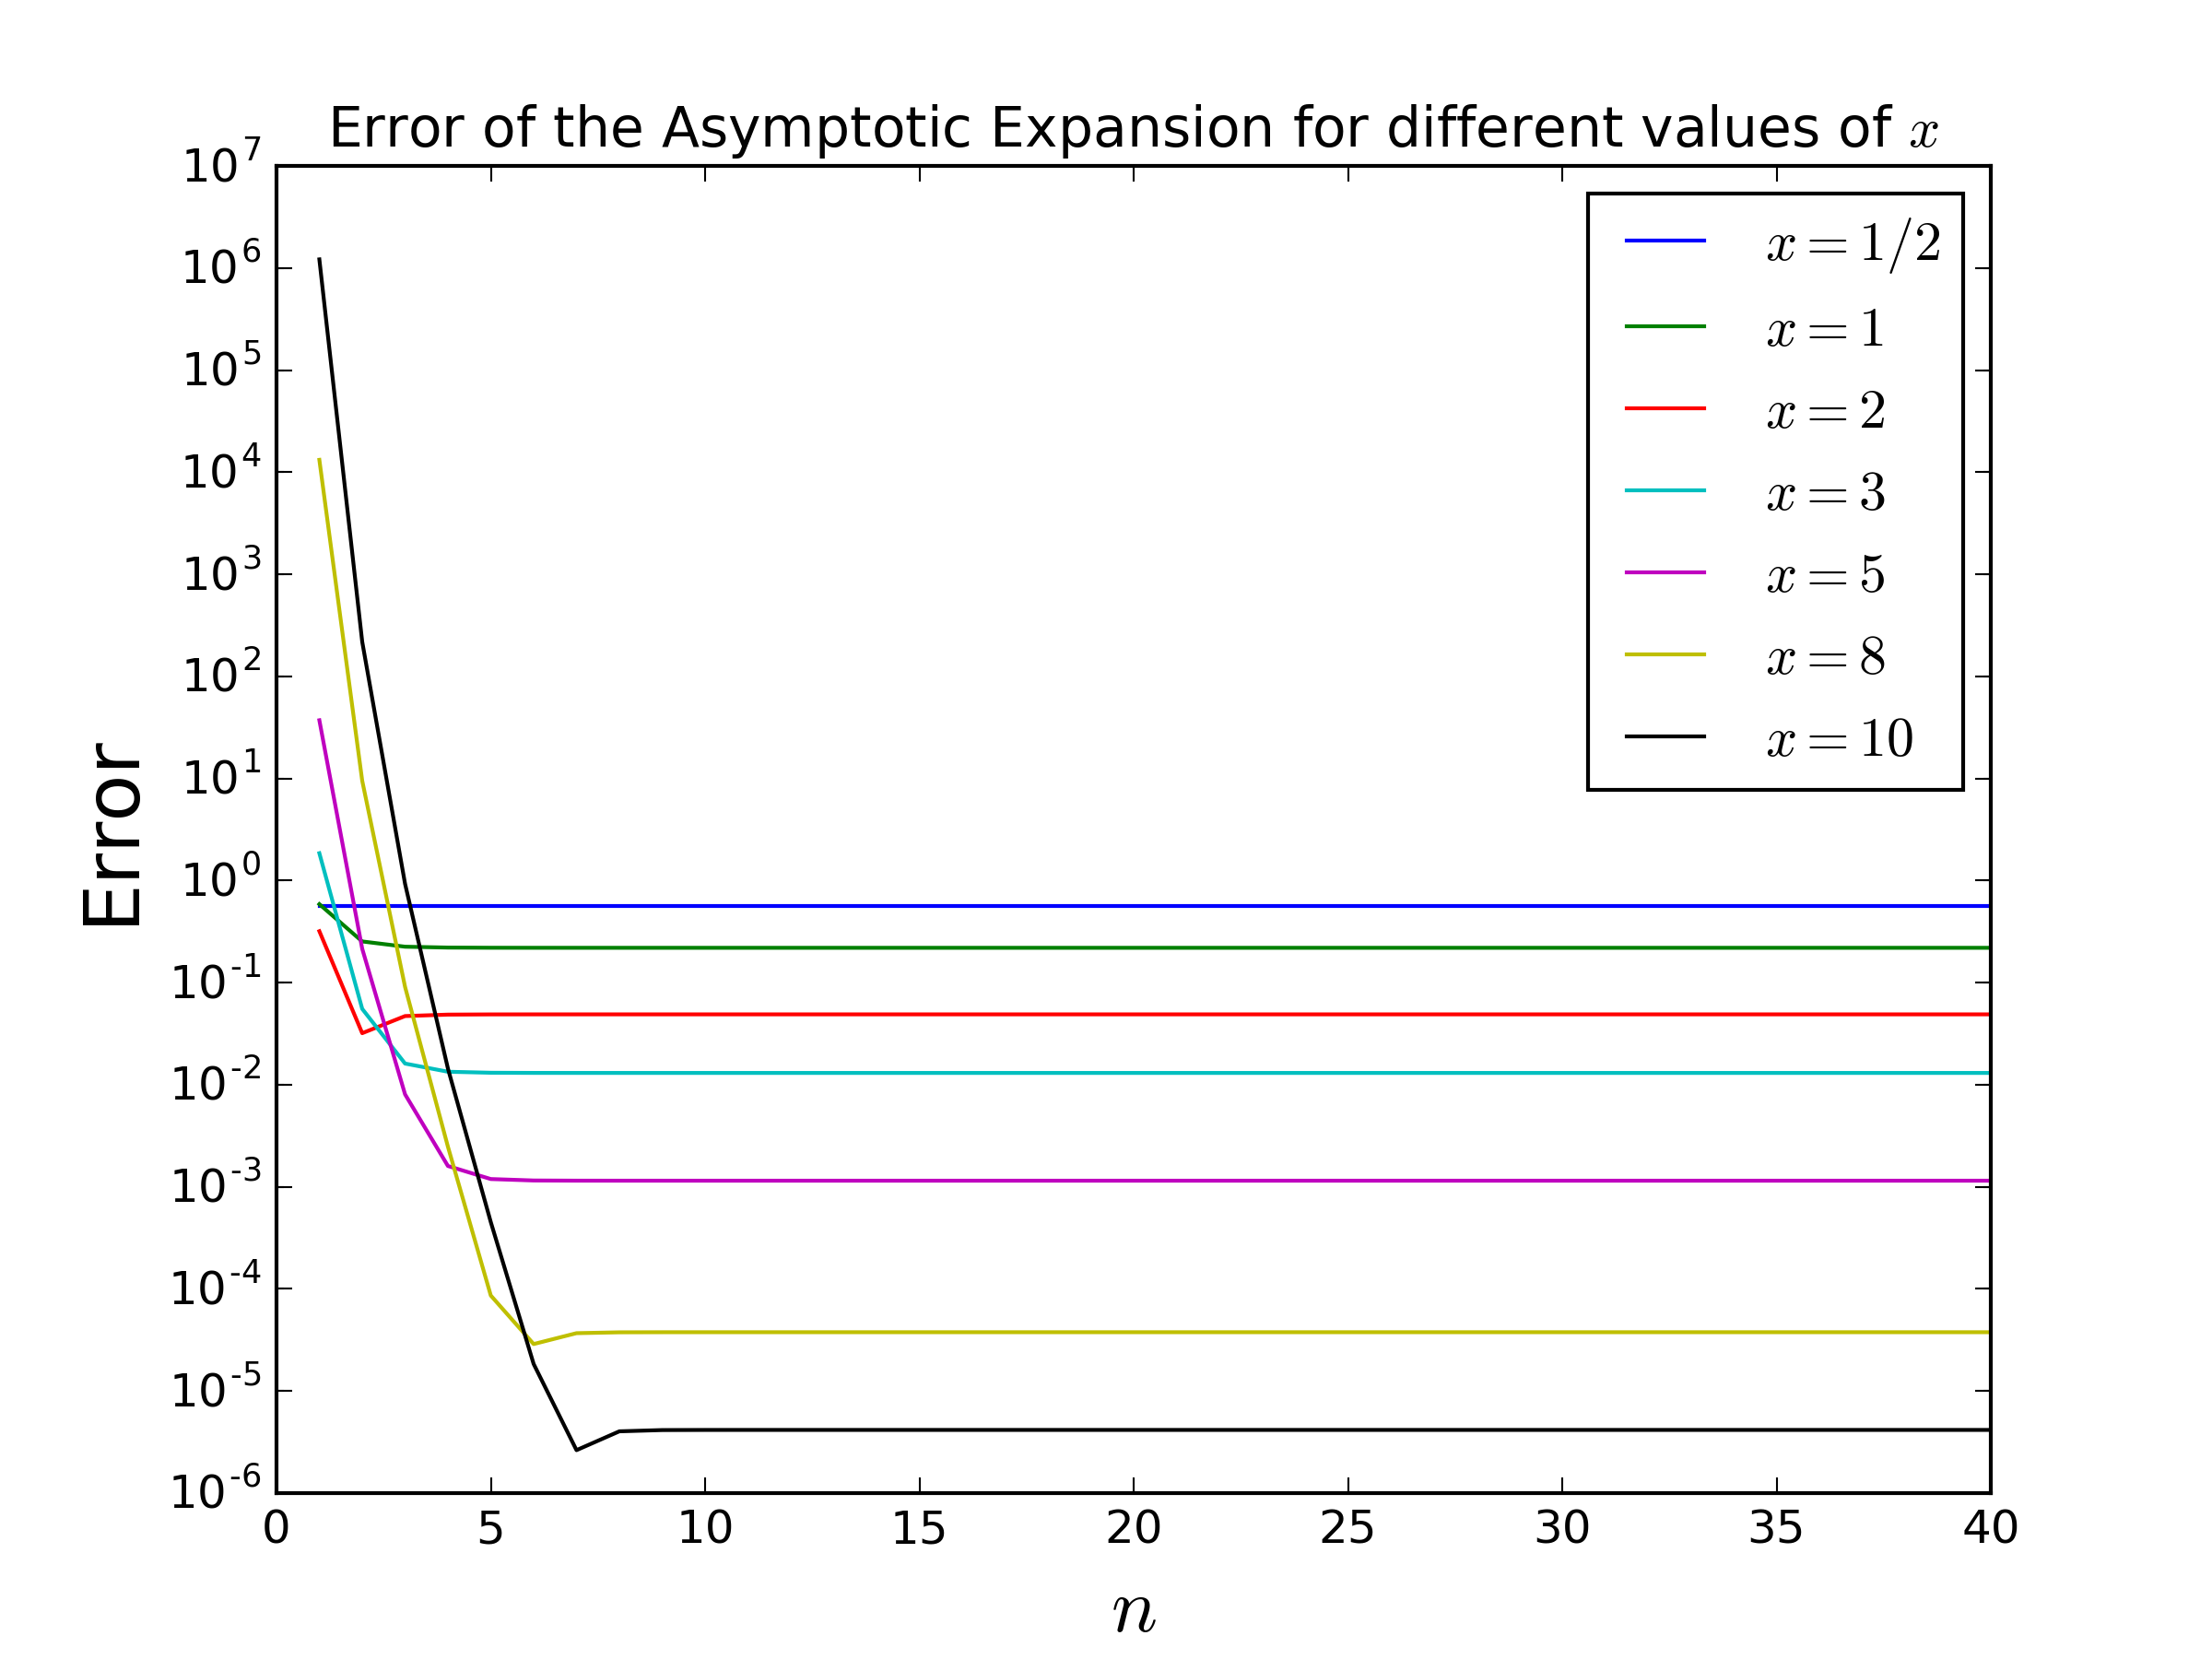
\includegraphics[width=\textwidth]{problem_2.png}
\end{figure}








\end{document}
